%cs-rd_intro.tex
\subsection{Wideband Compressed Sensing ADCs}\label{sct:wideband_cs_adc}
Sampling rate is crucial to signal processing systems since high clock rate enhances the power consumption and increases the burden of data transmission and storage. However, it has long been bounded by the Nyquist theory which denotes the minimum sampling rate for traditional acquisition methods, and couldn't reduced easily. In order to overcome this problem, recently many signal processing devices embed CS into analog-to-digital converters (ADCs) and successfully reduces the size of measurements and thus releases the limitation given by the Nyquist theory. As a consequence, the new systems using a relatively lower clock rate significantly outperform the traditional acquisition systems.   

\subsubsection{Random demodulator}
Random demodulator (RD)\cite{tropp2010beyond} is one of the most popular analog-to-digital converters for CS-based signal acquisition and processing. It develops the stability and robustness of CS measurement, and achieves a sub-Nyquist rate ADC for signal sampling and sequentially enhances the system power efficiency.  

\begin{figure}[!b]
\centering
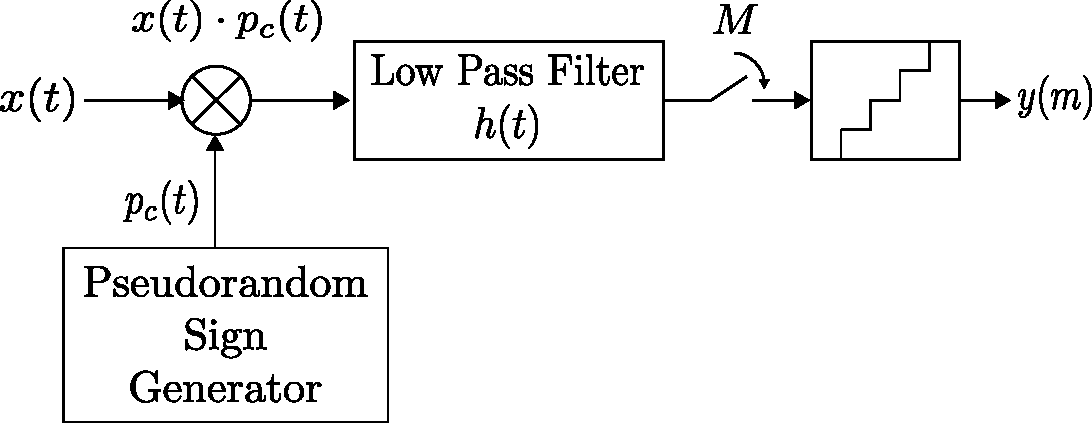
\includegraphics[width=3.2in]{pictures/random_demodulator.pdf}
\DeclareGraphicsExtensions.
\caption{Block diagram of random demodulator (RD). The components includes a pseudo-random sign generator, a low-pass filter, and a sub-Nyquist ADC}\label{RD}
\end{figure}

Figure \ref{RD} shows the construction of the random demodulator: It consists of a pseudo-random sign generator, a low-pass filter, and a sub-Nyquist ADC. The input $K$ sparse signal is first mixed with the chipping sequence $p_c(t)$ which is a waveform and constructed by pseudo-random variables of $\{\pm 1\}$. This chipping sequence is generated by the pseudo-random sign generator which alternates at the Nyquist rate $N$. The mixed production $x(t) \cdot p_c(t)$ then passes through a low pass filter $h(t)$ for anti-aliasing, and finally is sampled by a ADC uniformly at the rate of $m = O(K\log(N/K)) << N$. %N = W , R = M

\subsubsection{Modulated Wideband Convertor}
In the cases of sampling a multi-band signals whose carrier frequencies are unknown or time-variant (blind multi-band signal receiving), the main task is to design a receiver working independently on the carrier frequency at a low rate\cite{mishali2009blind}. Recently, a novel architecture termed modulated wideband converter (MWC) is developed, which applies the CS theory to the traditional blind multi-band signal receivers based on non-uniform sampling\cite{black1980time}. This innovative architecture successfully provides a minimal requirement for the size of observations\cite{mishali2010theory} thus decrease the power consumption.

\begin{figure}[!t]
\centering
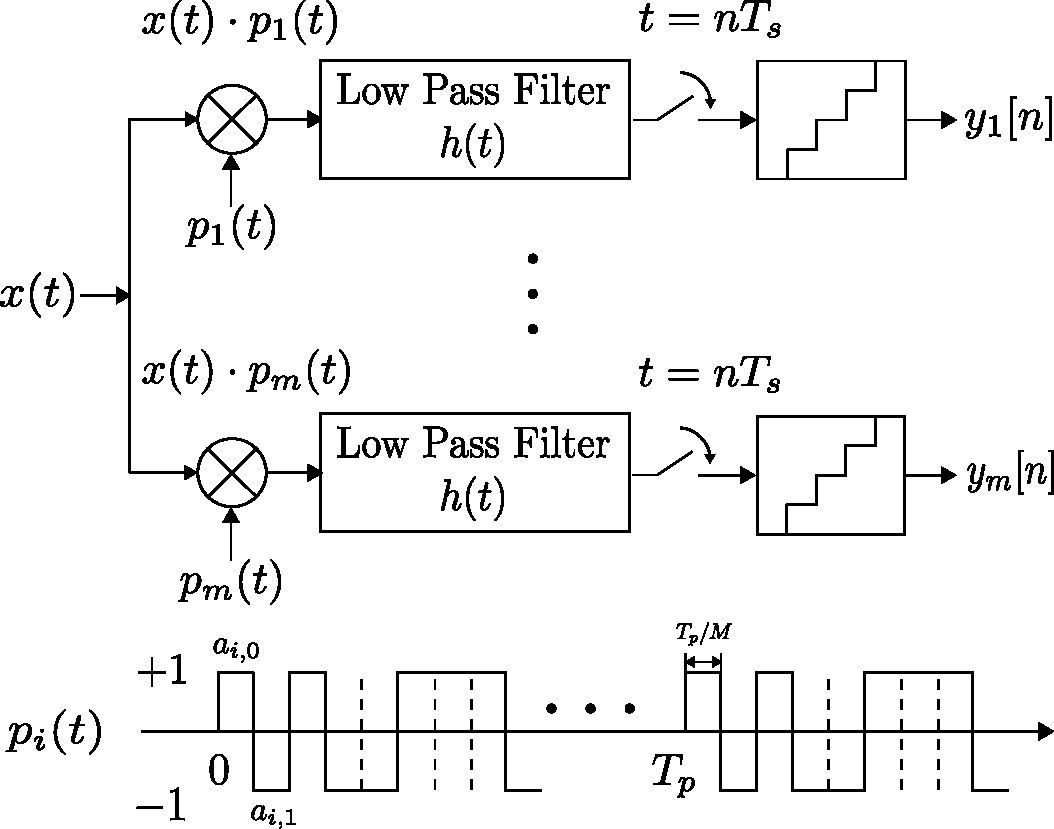
\includegraphics[width=3.2in]{pictures/MWC1.pdf}
\DeclareGraphicsExtensions.
\caption{Block diagram of modulated wideband convertor (MWC). The components includes parallel periodic waveforms mixers, low-pass filters, and sub-Nyquist ADCs}\label{MWC1}
\end{figure}

The MWC consists of groups of periodic waveforms, low pass filters and sub-Nyquist rate ADCs, and can be treated as a parallel structure of the random demodulator (RD). As shown in Figure \ref{MWC1}, each group of periodic sequence $p_i(t)$ with minimum interval of $T_p/M$ mixes the input multi-band signal $x(t)$ for shifting the spectrum by $\Delta f_p$ ($f_p = 1/{T_p}$ is the frequency of $p_i(t)$) and filtering it to the baseband for sampling. In the end, low rate ADCs sample the mixed productions at a rate $f_s$ far less than the Nyquist rate $f_{NYQ}$.

Considering the CS measurement MWC, recovering the $\mathbf z(f)$ where each row $X(f-lf_p)$ presents sparse spectrum segments can be regarded as recovering a infinite set of joint sparse vectors. This problem can be solved by changing it to the problem of multiple measurement vectors (MMV)\cite{mishali2008reduce} and has been implemented. 

\subsubsection{CS based signal processing}
Considering that many signal processing applications such as detection, classification, estimation and filtering do not require entire signal reconstruction, and only parts of certain information from measurements are needed, thus we prefer to filter out the useless information before further signal processing. Therefore, if we could estimate the useless information corresponding to some observations $y_I$, and then $throw$ them $away$ before CS based signal recovery, we can avoid a high computational complexity and thus save the power efficiency significantly. This novel idea comes from the compressive signal processing (CSP)\cite{davenport2010signal}.

\subsubsection{Non-Uniform Sampling}
The non-uniform sampling aims at sampling signals in a local Fourier sparse representation\cite{rauhut2010compressive} (LFS) (e.g. wideband signals), and provides an non-uniformly sampling pattern at pseudo-random time points with a low average rate, which establishes a sensing matrix $A$ which can be regarded as a random partial Fourier matrix $F_{T}$ that consists of randomly chosen columns of the discrete Fourier matrix(DFT) and indexed by $T$. According to \cite{ragheb2007implementation}, the matrix $A$ satisfies the RIP in compressive sensing so the acquisition model produces a stable reconstruction of $\hat s$ via $l1$-minimization using $m \geq O(slog(N/s))$ samples\cite{ragheb2007implementation}. 
